\chapter{Tight binding model}
	For electrons in a periodical lattice that are strongly bound to positive ions, as for lower orbital ones, we can use the tight binding model to calculate the band structure. \\
	We will start with a general derivation of the tight binding approximation and finish with an analytical solution of the nearest neighbor tight binding of graphene.
		
	\section{Tight binding model}
		The one electron Hamiltonian labeled by l is given by
		\begin{equation}
			\hat H_l = - \frac{\hbar^2}{2m_e} \nabla_l^2 + \sum_{j=1}{N}(\vec{r_l - R_j}),
		\end{equation}
		where we are regarding a Bravais lattice, with positive ions on the positions $\vec{R_j}$ and N as number of lattice sites. The Hamiltonian of all electrons is therefore given by : 
		\begin{equation}
			\hat H = \sum_{j=1}^{N} \hat H_l.
		\end{equation}
		In the \textit{tight binding model} each electron is "tightly" bound to a particular lattice site and can be described by
		\begin{equation}
			\hat H_l^a = - \frac{\hbar^2}{2m_e} \nabla_l^2 + V(\vec{r_l - R_l}).
		\end{equation}
		In addition we define the potential energy as $\Delta V = \sum_{j \neq l}^N V(\vec{r_l - R_j})$ from the other ions at sites $\vec{R_j}, j \neq l$, which can be treated pertubatively. While calculating the band structure of a lattice with more than one atom per unit cell (as for example of graphene) we need to notice that translating the sub-lattice A into B is not a symmetry operation. As a consequence we have to treat the different sub-lattices apart by linearizing the trial wave-function. For two atoms per unit cell, like in the honeycomb lattice from graphene, we may write down the trial wave-function as :
		\begin{equation}
			\label{eq:tightBindingPsiSum}
			\psi_\vec k (\vec{r}) = a_\vec k  \psi_\vec k^{(A)} (\vec r) + b_\vec k \psi_\vec k^{(B)}(\vec r),
		\end{equation}
		where A and B represent the sub-lattices and $a_\vec k$ and $b_\vec k$ are complex functions of $\vec k$. $\psi_\vec k^{(A)}$ and $\psi_\vec k^{(B)}$ are Bloch functions and may be written as : 
		\begin{equation}
			\label{eq:tightBindingBlochWave}
			\psi_\vec k^{(j)}(\vec r) = \sum_{\vec R_l} e^{i \vec{k \cdot R_l}} \phi^{(j)}(\vec{r} + \boldsymbol{\delta_j} - \vec{R_l})
		\end{equation}
		with $\delta_j$ as vector connecting the two sub-lattices. For a better understanding we shortly want to prove the Bloch compatibility of the last relation
		\begin{equation}
			\begin{split}
				\psi(\vec{r + R}) &= \sum{R_l} e^{i \vec{k \cdot R_l}} \phi(\vec{r + R} + \boldsymbol{\delta_j} - \vec{R_l}) \\
				&=  e^{i \vec{k \cdot R}}\sum{R_l} e^{i \vec{k \cdot R_l - R}} \phi(\vec{r} + \boldsymbol{\delta_j} - (\vec{R_l - R} )) \\
				&= e^{i \vec{k \cdot R}}\sum{R_l} e^{i \vec{k \cdot R'}} \phi(\vec{r} + \boldsymbol{\delta_j} - \vec{R'} ) \\
				&= e^{i \vec{k \cdot R}} \psi(\vec r + \boldsymbol \delta_j).
			\end{split}				
		\end{equation}
		The next aim is to find a general solution for the Schrödinger equation
		\begin{equation}
			\hat H | \psi_\vec k \rangle = \epsilon_\vec k | \psi_\vec k \rangle
		\end{equation}
		of the tight binding model. Multiplying the above equation by $\langle \psi_\vec k^* |$ yields
		\begin{equation}
			\langle \psi_\vec k^* | \hat H | \psi_\vec k \rangle = \epsilon_\vec k \langle \psi_\vec k | \psi_\vec k \rangle,
		\end{equation}
		which can be rewritten in matrix form with the help of Eq. \ref{eq:tightBindingPsiSum}.
		\begin{equation}
			\begin{pmatrix}
				a_\vec k^* & b_\vec k^*
			\end{pmatrix}
			 H_\vec k 
			 \begin{pmatrix}
				a_\vec k \\
				b_\vec k
			 \end{pmatrix}
			 = \epsilon_\vec k 
			 \begin{pmatrix}
				a_\vec k^* & b_\vec k^*
			 \end{pmatrix}
			  S_\vec k 
			 \begin{pmatrix}
			 	a_\vec k \\
				b_\vec k
			\end{pmatrix}
		\end{equation}
		with the Hamiltonian matrix defined as
		\begin{equation}
			H_\vec k \equiv 
			\begin{pmatrix}
				\psi_\vec k^{(A)*} \hat H \psi_\vec k^{(A)} & \psi_\vec k^{(A)*} \hat H \psi_\vec k^{(B)} \\
				\psi_\vec k^{(B)*} \hat H \psi_\vec k^{(A)} & \psi_\vec k^{(B)*} \hat H \psi_\vec k^{(B)}
			\end{pmatrix}
			= H_\vec k^\dagger
		\end{equation}
		and the overlap matrix
		\begin{equation}	  
			S_\vec k \equiv 
			\begin{pmatrix}
				\psi_\vec k^{(A)*} \psi_\vec k^{(A)} & \psi_\vec k^{(A)*} \psi_\vec k^{(B)} \\
				\psi_\vec k^{(B)*} \psi_\vec k^{(A)} & \psi_\vec k^{(B)*} \psi_\vec k^{(B)}
			\end{pmatrix}
			= S_\vec k^\dagger,
		\end{equation}
		that needs to be included because of the non orthogonality of the wave function $\psi_\vec k$. The eigenfunctions can now be obtained by the secular equation :
		\begin{equation}
			det[H_\vec k - \epsilon_\vec k^\lambda S_\vec k] = 0
		\end{equation}
		With help of Eq. \ref{eq:tightBindingBlochWave} we can rewrite the matrix entries of the Hamiltonian matrix into
		\begin{align}
			\label{eq:tightHij}
			H_\vec k^{ij} &= \sum_{\vec{R_l, R_m}} e^{i \vec{k \cdot (\vec{R_l - R_m)}}} \int d^2 r \phi^{(i)*}(\vec{r } + \boldsymbol{\delta_i} - \vec{R_l}) H \phi^{(j)}(\vec{r} + \boldsymbol{\delta_i} - \vec{R_m}) \\
			&= N \sum_{\vec R_l} e^{i \vec{k \cdot R_l}} \int d^2 \phi^{(i)*}(\vec r)[H^a + \Delta V] \phi^{(j)}(\vec{r} + \boldsymbol{\delta_{ij}} - \vec{R_l}) \\
			&= N (\epsilon^{(i)} s_\vec k^{ij} + t_\vec k^{ij}),
		\end{align}
		where $\delta_{ij} \equiv \delta_j - \delta_i$,
		\begin{equation}
			\label{eq:tightSij}
			s_\vec k^{ij} \equiv \sum_{\vec R_l} e^{i \vec{k \cdot R_l}} \int d^2 r \phi^{(i)*}(\vec{r} + \boldsymbol{\delta_i} - \vec{R_k}) \phi^{(j)}(\vec{r} + \boldsymbol{\delta_j} - \vec{R_mk}) = \frac{S_k^{ij}}{N}
		\end{equation}
		and the so called hopping matrix is defined as
		\begin{equation}
			t_\vec k^{ij} = \sum_{\vec R_l} e^{i \vec{k \cdot R_l}} \int d^2 r \phi^{(i)*}(\vec{r} + \boldsymbol{\delta_i} - \vec{R_k}) \Delta V \phi^{(j)}(\vec{r} + \boldsymbol{\delta_j} - \vec{R_m})
		\end{equation}
		The secular equation now reads :
		\begin{equation}
			\label{eq:generalTightBindingSolution}
			det[t_\vec k^{ij} - \epsilon_\vec k ^\lambda - \epsilon^{(i)}] = 0
		\end{equation}
		All of the atoms on the different sub-lattices have the same electronic configuration ($p_z$ orbitals) and therefore $\epsilon^{(i)} = \epsilon_0$ becomes a constant, which we will omit in future discussions.
					
	\section{Nearest neighbor tight binding for graphene}
		\begin{figure}[h]
			\centering
			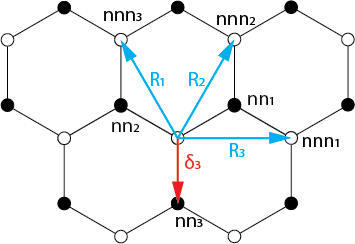
\includegraphics[width=0.5\textwidth]{figures/TightBinding/tightBinding.png}
			\caption{Nearest (nn) and Next nearest neighbors (nnn) of a carbon atom in the hexagonal lattice.$\vec R_1$, $\vec R_2$ and $\vec R_3$ connect the centered lattice site to its next nearest neighbors. $\boldsymbol{\delta_3}$ is the connection vector between the A and the B sublattice. The nearest neighbor vectors can be build from the next nearest neighbor vectors.}
			\label{fig:tighBindingHoneycomb}
		\end{figure}
		Having found a general solution, we continue deriving a specific one for graphene with its honeycomb lattice. The connection vectors to the next nearest and the nearest neighbor are given in Fig: \ref{fig:tighBindingHoneycomb}.
		\begin{align}
			\label{eq:tightBindingVectors}
			\vec R_1 = \frac{a}{2} 
			\begin{pmatrix} 
				\sqrt{3} \\
			 	3
			 \end{pmatrix} & 
			 \vec R_2 = \frac{a}{2} 
			 \begin{pmatrix} 
			 	3 \\
			 	- \sqrt{3}
			 \end{pmatrix}
			 \vec R_3 = a 
			 \begin{pmatrix} 
			 	\sqrt{3} \\ 
			 	0
			 \end{pmatrix} &
			 \boldsymbol{\delta_3} = a \begin{pmatrix} 0 \\ -1\end{pmatrix}
		\end{align}
		We start with the secular equation (\ref{eq:generalTightBindingSolution}) and neglect the energy shift $\epsilon_0$, which only contains a shift in the energy.
		\begin{equation}
			\begin{pmatrix}
				H_k^{AA} - \epsilon s_k^{AA} & 	H_k^{AB} - \epsilon s_k^{AB} \\
				H^{BA} - \epsilon s_k^{BA} & 	H_k^{BB} - \epsilon s_k^{BB}
			\end{pmatrix}
		\end{equation}
		With the given variables $H^{ij}$ and $S^{ij}$. Equation \ref{eq:tightHij} can be rewritten under the graphene double sub-lattice conditions as:
		\begin{equation}
			H_k^{ij} = t_k^{ij}
		\end{equation}
		The N cancels from the sum over the lattice sites and $\epsilon^{(i)}$ is omitted. In addition on can write: 
		\begin{equation}
			\begin{split}
				H_k^{AA} = t_k^{AA} &= \sum_{\vec R_1}^{\vec R_l} e^{i \vec{k \cdot R_l}} \underbrace{\int d^2 r \phi^{(A)*}(\vec{r}) \Delta V \phi^{(A)}(\vec{r} + \boldsymbol{\delta_3}}_{t_{nnn}} \\ 
				 &= t_{nnn} (e^{i \vec{k \cdot R_1}} + e^{-i \vec{k \cdot R_1}} + e^{i \vec{k \cdot R_2}} + e^{-i \vec{k \cdot R_2}} + e^{i \vec{k \cdot R_3}} + e^{-i \vec{k \cdot R_3}}) \\
				 &= 2t_{nnn} ( \sum_{i=1}^{3} cos(\vec{k \cdot R_i}))	= t_k^{BB}
			\end{split}			
		\end{equation}
		\begin{equation}
			\begin{split}		
				H_k^{AB} = t_k^{AB} &= \sum_{\vec R_1}^{\vec R_3} e^{i \vec{k \cdot R_l}} \underbrace{\int d^2 r \phi^{(A)*}(\vec{r}) \Delta V \phi^{(B)}(\vec{r} + \boldsymbol{\delta_j})}_{t} \\
				&= t(1 + e^{i \vec{-k \cdot \vec{R_1}} + e^{-i \vec{k \cdot R_3}}}) 	\\
				&= (t_k^{BA})^*	
			\end{split}			
		\end{equation}
		Eq. \ref{eq:tightSij} can now be transformed to
		\begin{equation}
				s_k^{AA} = s_k^{BB} = 1	
		\end{equation}
		due to the normalizations of the atomic wave-functions ($\int d^2 r \phi^{(j)*}(\vec r) \Delta V \phi^{(j)}(\vec r) = 1$) we have
		\begin{equation}
			\begin{split}
				s_k^{AB} &= \sum_{\vec R_l} e^{i \vec{k \cdot R_l}} \underbrace{\int d^2 r \phi^{(A)*}(\vec{r}) \phi^{(B)}(\vec{r} + \boldsymbol{\delta_3})}_{s} \\
				&= s(1 + e^{i \vec{k \cdot R_1}} + e^{i \vec{k \cdot R_3}})	\\
				&= (s_k^{BA})^*.			
			\end{split}
		\end{equation}
		Having all the tools to calculate the energy $\epsilon$ we define 
		\begin{equation}
			\gamma_k = 1 + e^{i \vec{k \cdot R_1}} + e^{i \vec{k \cdot R_1}} 
		\end{equation}
		Therefore the above equations  turn into
		\begin{align}
			t_k^{AB} = t \gamma_k^* = (t_k^{BA})^* \\
			s_k^{AB} = s \gamma_k^* = (s_k^{BA})^*.
		\end{align}
		For the final secular equation we obtain
		\begin{equation}
			det
			\begin{pmatrix}
				t_k^{AA} - \epsilon_k & (t - s\epsilon_k)\gamma_k^* \\
				(t - s\epsilon_k)\gamma_k & t_k^{AA} - \epsilon_k
			\end{pmatrix}
			= 0
		\end{equation}
		with the solution
		\begin{equation}
			\label{eq:tightEnergyFrac}
			\begin{split}
				(t_k^{AA} - \epsilon_k)^2 &= (t - s \epsilon_k)^2|\gamma_k|^2 \\
				\pm t_k^{AA} - \epsilon_k &= \pm (t - s \epsilon_k)|\gamma_k| \\
				\pm \epsilon_k (\frac{1}{|\gamma_k|} - s)&= \pm t|\gamma_k| - t_k^{AA} \\
				\epsilon_k^{\pi \pm} &= \frac{t_k^{AA} \pm t|\gamma_k|}{1 \pm s|\gamma_k|}.
			\end{split}
		\end{equation}
		This expression may be expanded under the assumptions $s \ll 1$ and $t_{nnn} \ll t$. The needed Tayler expansion is given by
		\begin{equation}
			\begin{split}
				\mathcal{T}_1^0 &= \frac{1}{1+x} \\
				&= 1 - \frac{x}{(1+x)^2} 
			\end{split}	
		\end{equation}
		with $x = |\gamma_k|s$, because of the assumptions we can rewrite Eq. \ref{eq:tightEnergyFrac} into 
		\begin{equation}
			\label{eq:tightBindingAnalyticalSolution}
			\begin{split}
				\epsilon_k^{\pi \pm} &= t_k^{AA} + t|\gamma_k| - ts|\gamma_k|^2 \\
				&= 2t' ( \sum_{i=1}^{3} \cos(\vec{k \cdot R_i})) \pm t\sqrt{3 + 2\sum_{i=1}^{3} \cos(\vec{k \cdot R_i})},
			\end{split}
		\end{equation}
		where we defined $t' \equiv t_{nnn} - st$, while using $\vec{R_3} = \vec{R_2} - \vec{R_1}$ and
		\begin{equation}
			\begin{split}
					|\gamma_k| &= \sqrt{(1 + e^{i\vec{k \cdot R_1}} + e^{i\vec{k \cdot R_3}})(1 + e^{-i\vec{k \cdot R_1}} + e^{-i\vec{k \cdot R_3}})} \\
					&= \sqrt{1 + e^{-i\vec{k \cdot R_1}} + e^{-i\vec{k \cdot R_3}} + e^{i \vec{k \cdot R_1}} + 1 + e^{i \vec{ k \cdot (R_1 - R_3)}} + e^{i\vec{k \cdot R_3}} + e^{i \vec{k \cdot (R_3 - R_1)}} + 1} \\
					&= \sqrt{3 + 2\sum_{i=1}^{3} cos(\vec{k \cdot R_i})}.
			\end{split}
		\end{equation}
		Including the vectors given in equation \ref{eq:tightBindingVectors}, while using the addition theorem $\cos(x \pm y) = \cos(x)\cos(y) \mp \sin(x)\sin(y)$ one obtains :
		\begin{equation}
			\epsilon_k^{\pm \pi} = t'f_{nnn}(\vec k) \pm t\sqrt{3 + f_{nnn}(\vec k)}
		\end{equation}
		with
		\begin{equation}
			f_{nnn}(\vec k) = 2\cos(\sqrt{3} k_x a ) + 4\cos(\frac{3}{2} k_y a)\cos(\frac{\sqrt{3}}{2}k_x a).
		\end{equation} \\\\
		The analytical solution of the tight binding approximation in Equation \ref{eq:tightBindingAnalyticalSolution} will be used to make an accurate tight binding fit for the parameters t and t', with the results gained in our \textit{FPLO}-\textit{DFT} results. However, before the fitting we want to solve the tight binding approximation for some high symmetry points. \\
		\begin{compactenum}
			\item $\vec M \left(\frac{2\pi}{\sqrt{3}a}, 0\right)$:
				\begin{equation}
					\begin{split}
						f_{nnn} \left(\frac{2\pi}{\sqrt{3}a}, 0\right) &= 2 + 4 = 6 \\
						\Rightarrow \epsilon_\vec M^{\pm \pi} &= 6t'+ 3t
					\end{split} 
				\end{equation}
			\item $\vec K \left( \frac{2\pi}{\sqrt{3}3a}, \frac{2\pi}{3 a} \right)$:
				\begin{equation}
					\begin{split}
						f_{nnn} \left( \frac{2\pi}{\sqrt{3}3a}, \frac{2\pi}{3 a} \right) &= 2 \underbrace{\cos \left( \frac{2\pi}{3} \right)}_{= - \frac{1}{2}} + 4 \underbrace{\cos (\pi)}_{= -1} \underbrace{\cos \left( \frac{\pi}{3} \right)}_{\frac{1}{2}} = -3\\
						\Rightarrow \epsilon_\vec K^{\pm \pi} &= -3t' 
					\end{split}
				\end{equation}
			\item $\boldsymbol \Gamma (0,0):$
				\begin{equation}
					\begin{split}
						f_{nnn}(0,0) &= 2\cos(2\pi) + 4 \cos(\pi) = -2 \\
						\Rightarrow \epsilon_\vec M^{\pm \pi} &= -2t' \pm t
					\end{split}
				\end{equation}
		\end{compactenum}
		We can conclude that both bands have a symmetrical appearance for a fixed t' and that there exists a degenerated K point. Furthermore there is a band gap of 6t at the \textbf{M} point and 2t at the $\boldsymbol{\Gamma}$ point. We can display the approximation graphically in Figure \ref{fig:tightbinding3dplot}.
		\begin{figure}[h]
			\centering
			\includegraphics[width=1\textwidth]{figures/TightBinding/tightbinding3dplot.png}
			\caption{Electronic dispersion in the honeycomb lattice for finite values of $t'=0.2t$ and $t=2.7$ eV.}
			\label{fig:tightbinding3dplot}
		\end{figure}
		
	\section{Tight binding fit for graphene}
		\begin{figure}[h]
			\centering
			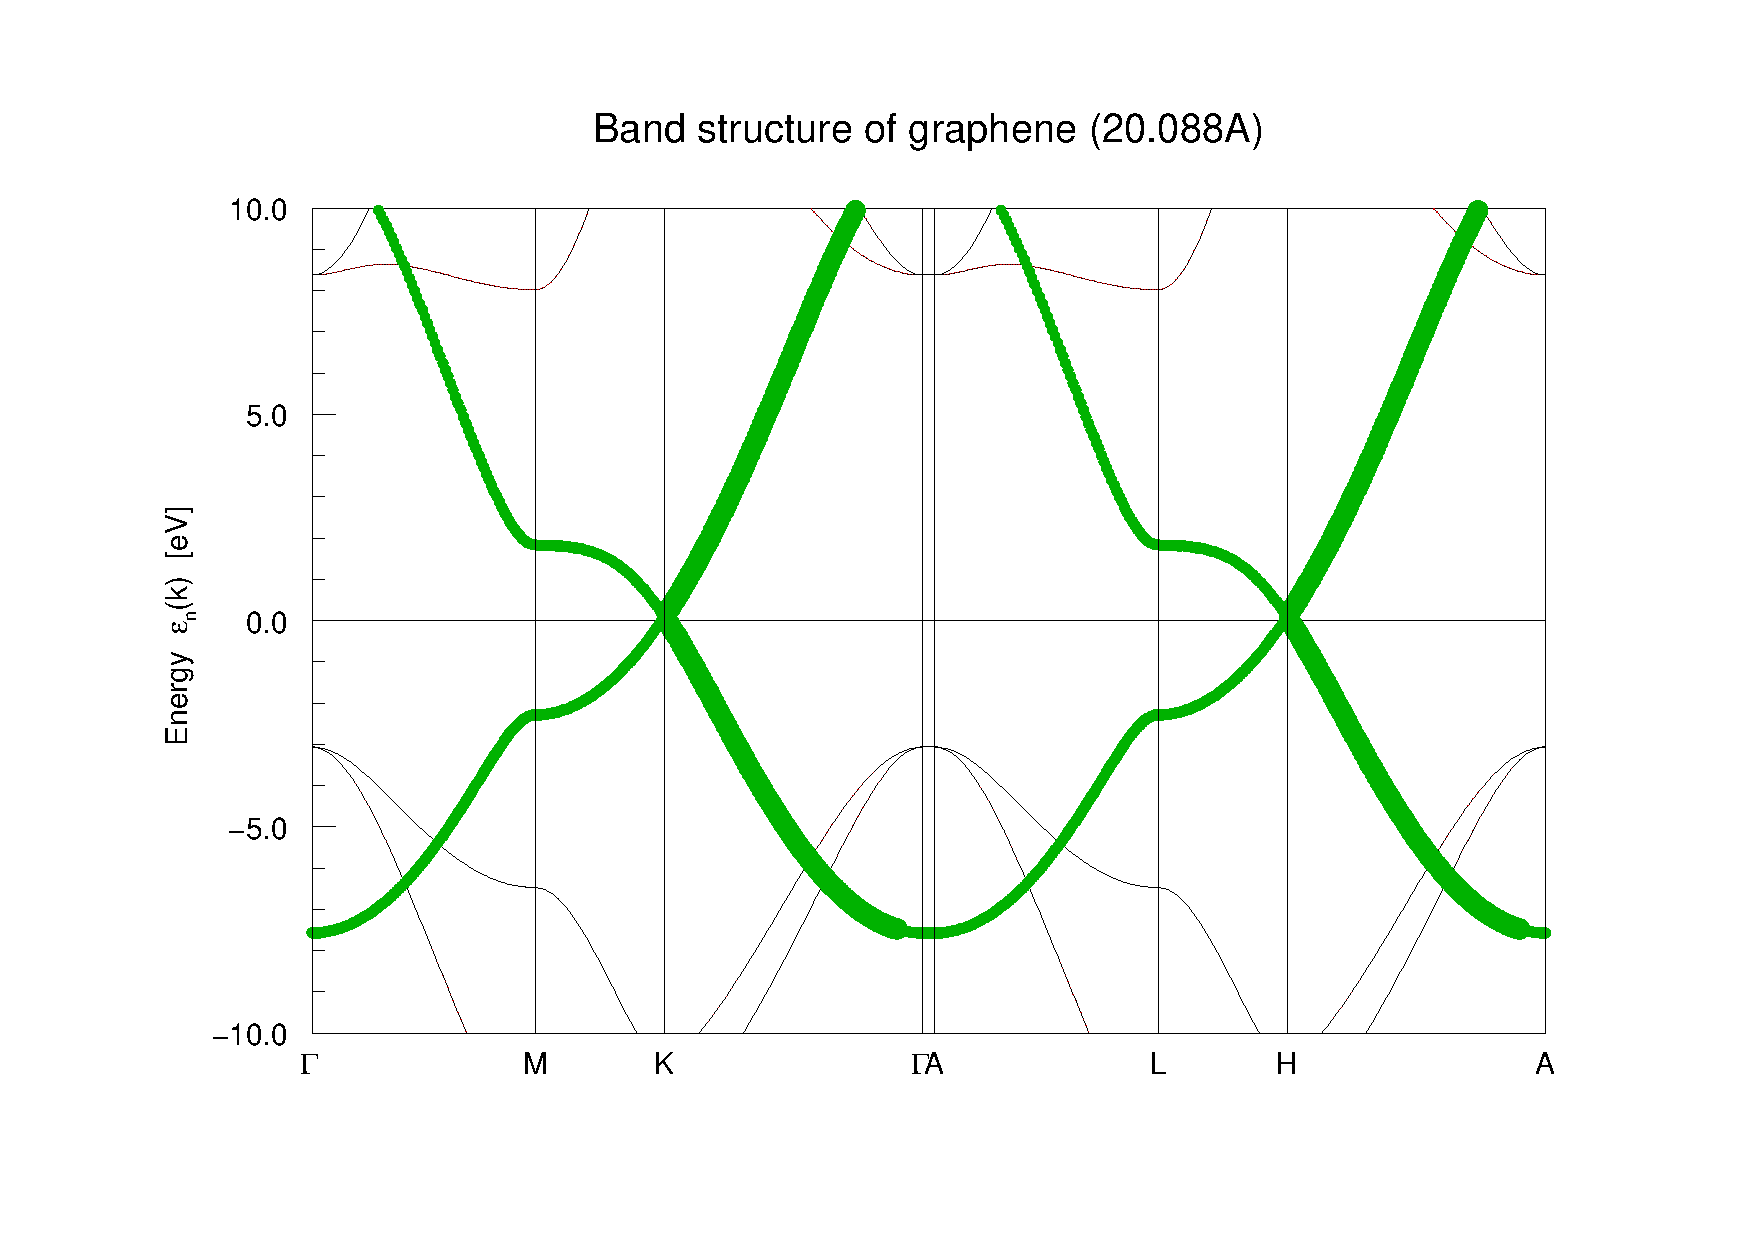
\includegraphics[width=1\textwidth]{figures/TightBinding/tightBindingPiGraphene.pdf}
			\caption{$\pi$-bands of graphene (green).}
			\label{fig:graphenePiBands}
		\end{figure}
		The fits for our analytical solution (Equation \ref{eq:tightBindingAnalyticalSolution}) are displayed in Figure \ref{fig:piPlusFit} and \ref{fig:piMinusFit}. We fitted over the general k-path including the high-symmetry points used in our previous band structure plots (Table \ref{table:highsymmetryPointsGraphene}, $\Gamma \rightarrow M \rightarrow K \rightarrow \Gamma \rightarrow A \rightarrow L \rightarrow L \rightarrow H \rightarrow A$, displayed with band weighting in Figure \ref{fig:graphenePiBands}). The fitting parameters were calculated from the FPLO-DFT data, by minimizing the variation:
		\begin{equation}
			\sigma = \sqrt{\left( \epsilon_{k}^{\pm \pi} - \epsilon_{FPLO} \right)^2},
		\end{equation}
		where $\epsilon_{k}^{\pm \pi}$ is the computed energy and $\epsilon_{FPLO}$ is the energy, with the same $\vec k$ value, taken from the FPLO-DFT. \\\\
		To fit the $\pi$-bands we first need to separate them from all other orbitals, by using the '+bweights' file of FPLO. In addition we have to transform the FPLO coordinates into physical coordinates used in our analytical solution. FPLO uses the latice vectors $\vec g_1$, $\vec g_2$ and $\vec g_3$ given in our transformation matrix
		\begin{equation}
			H =
			\begin{pmatrix}
				\vec g_1 \\
				\vec g_2 \\
				\vec g_3			
			\end{pmatrix}	
			= 
			\begin{pmatrix}
				0.248795 & 0.1243976 & 0 \\
				0 & 0.21546303 & 0 \\
				0 & 0 & 0.013714758
			\end{pmatrix}.
		\end{equation}
		\newpage
		If $\vec v$ is a vector in the FPLO coordinates $\vec v' = T^{-1} \vec v$ is a vector in the physical coordinates. Furthermore we have $H \vec v' = \vec v''$. Hence if we want to obtain $\vec v''$ in coordinates of our analytical solution, with the given Bravais vectors $\vec R_i$ transformed to reciprocal vectors $\vec b_i$
		\begin{equation}
			B = 
			\begin{pmatrix}
				\vec b_1 \\
				\vec b_2 \\
				\vec b_3
			\end{pmatrix}
			=
			\begin{pmatrix}
				\frac{2\pi}{3} & \frac{2\pi}{3} & 0 \\
				\frac{2\pi\sqrt{3}}{3} & -\frac{2\pi \sqrt{3}}{3} & 0 \\
				0 & 0 & 1
			\end{pmatrix}
			= 
			\begin{pmatrix}
				2.0943951 & 2.0943951 & 0 \\
				3.62759873 & -3.62759873 & 0 \\
				0 & 0 & 1
			\end{pmatrix},
		\end{equation}
		\begin{equation}
			\vec v'' = H \vec v' = H T^{-1} \vec v = D \vec v.
		\end{equation}
		Having still the problem, that the unit length of $\vec g_i$ and $\vec b_i$ are different, we need to find the scaling factor s, by dividing the magnitudes 
		\begin{equation}
			s = \frac{|\vec b_1|}{|\vec g_1|} \approx 16.8363188,
		\end{equation}
		yielding
		\begin{equation}
			H' = 
			\begin{pmatrix}
				4.1887902 & 2.09439678 & 0 \\
				0 & 3.627260276 & 0 \\
				0 & 0 & 1
			\end{pmatrix}
		\end{equation}
		\begin{equation}
			D' = H' T^{-1} = H' S^{-1} H^{-1} = 
			\begin{pmatrix}
				3.6275987255 & 0 & 0 \\
				0 & 3.52760276 & 0 \\
				0 & 0 & 16.358306
			\end{pmatrix}.
		\end{equation}
		As s is diagonal we can rewrite D'
		\begin{equation}
			D'= H'H^{-1} S^{-1}
		\end{equation}
		The z-components are irrelevant and can be chosen arbitrarily. Remaining is then a rescaling of the k vectors used in FPLO of
		\begin{equation}
			D' = c \mathbbm{1}, c = \frac{|\vec b_1|}{|\vec g_1|} \frac{1}{| \vec a_1 |} = 3.6278976
		\end{equation}
		\\\\
		Examine the plots (Figures \ref{fig:piPlusFit} and \ref{fig:piPlusFit}) and the sigma values (Table \ref{table:tightBindingFit}) we notice, that fitting the $\pi_-$ band is for our chosen, very universal, path more accurate than the the $\pi_+$ band. The $\pi_-$ fit can reproduce the solutions of the FPLO-DFT very well, while the $\pi_+$ band has problems, especially between 0.6 - 1 and 2.3 - 2.6 k-values. The the difference of the two sigma values is 192.37 eV, i.e. the $\pi_-$ fit is 3.4 times better than the $\pi_+$ one.
		\begin{table}[h]
			\centering
			\begin{tabular}{cccc}
			     & t & t' & $\sigma$ \\
				\midrule
				 $\pi_+$ & 1.54 & -1.09 & 272.89 eV \\
				 $\pi_-$ & -1.35 & -0.59 & 80.52 eV\\
				\bottomrule
			\end{tabular}
			\caption{Fitted parameters t and t' with their variances for the graphene nearest-neighbor tight binding model.}
			\label{table:tightBindingFit}
		\end{table}
		\begin{figure}[h]
			\centering
			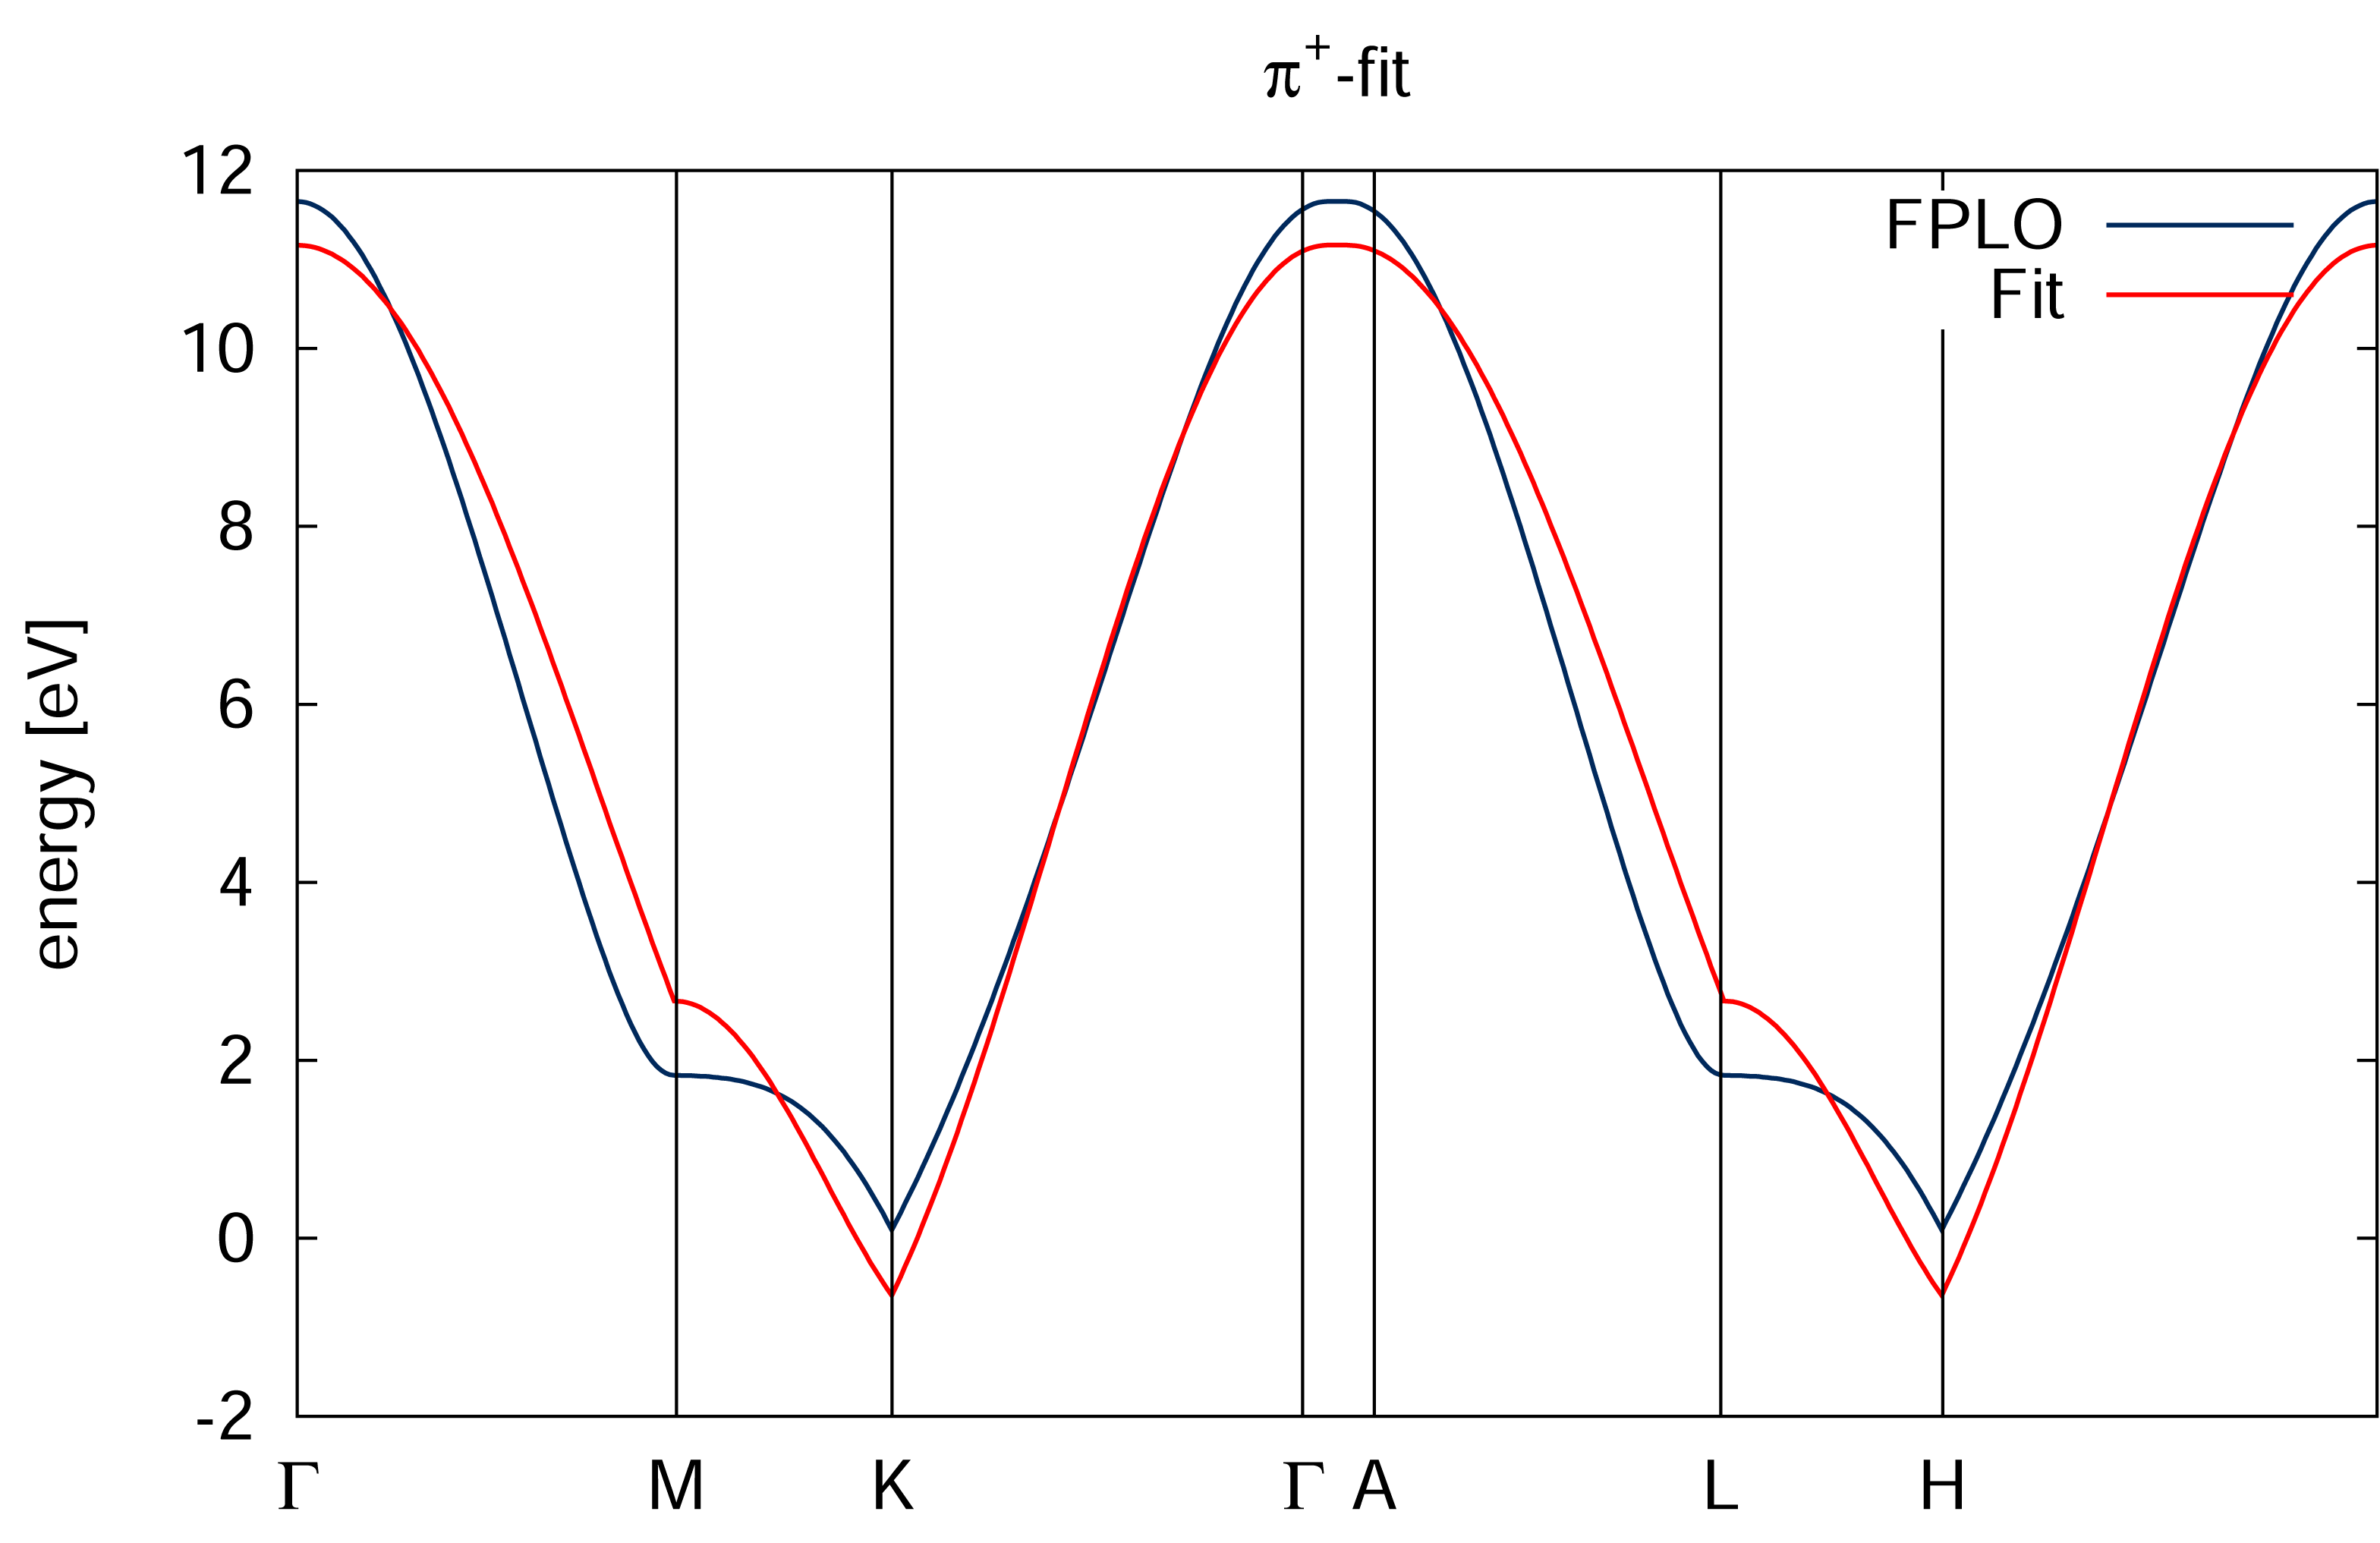
\includegraphics[width=1\textwidth]{Results/Figures/piPlusFit.png}
			\caption{$pi^+$-fit of the nearest neighbor tight binding model for graphene.}
			\label{fig:piPlusFit}
		\end{figure}
		\begin{figure}[h]
			\centering
			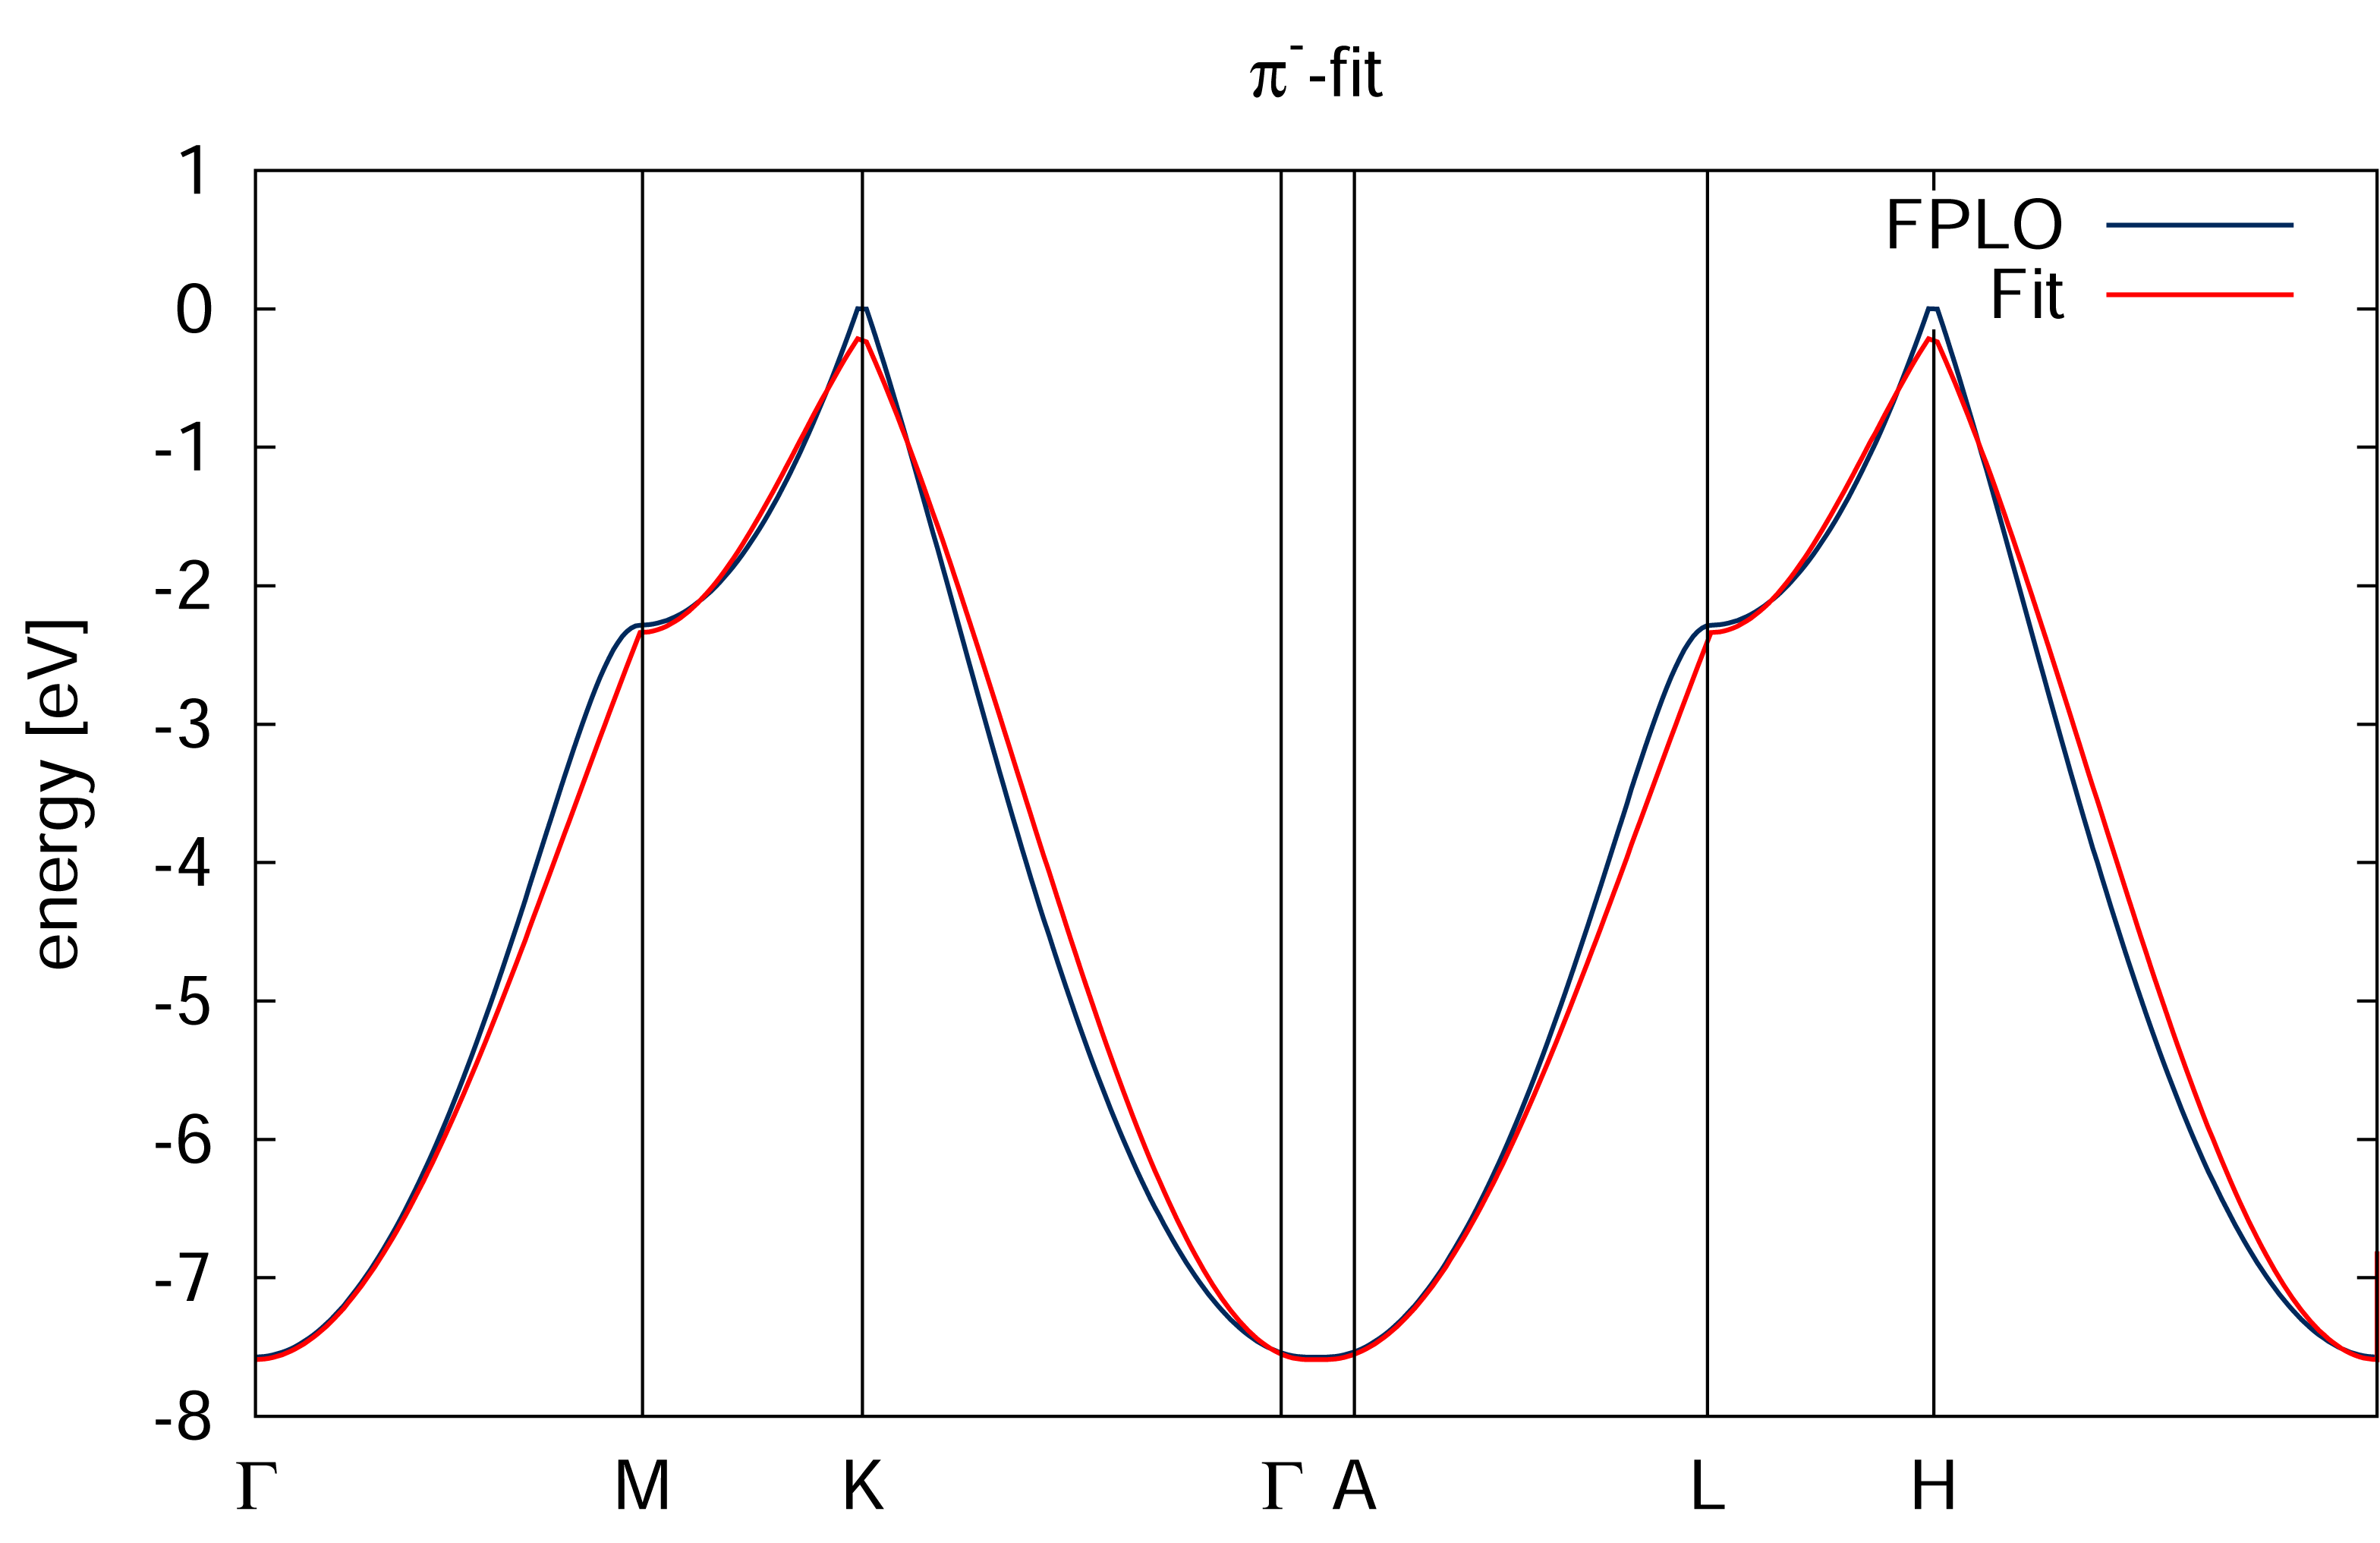
\includegraphics[width=1\textwidth]{Results/Figures/piMinusFit.png}
			\caption{$pi^-$-fit of the nearest neighbor tight binding model for graphene.}
			\label{fig:piMinusFit}
		\end{figure} \\\\
		The code used for the calculation is found in the appendix. 
		
		
	
 
		
	
	
	
	